\documentclass[xetex,mathserif,serif]{beamer}
\usepackage{polyglossia}
\setdefaultlanguage[babelshorthands=true]{russian}
\usepackage{minted}
\usepackage{tabu}

\useoutertheme{infolines}

\usepackage{fontspec}
\setmainfont{FreeSans}
\newfontfamily{\russianfonttt}{FreeSans}

\definecolor{links}{HTML}{2A1B81}
\hypersetup{colorlinks,linkcolor=,urlcolor=links}

\setbeamertemplate{blocks}[rounded][shadow=false]

\setbeamercolor*{block title alerted}{fg=red!50!black,bg=red!20}
\setbeamercolor*{block body alerted}{fg=black,bg=red!10}

\tabulinesep=1.2mm

\title{Визуальное моделирование, UML}
\author[Юрий Литвинов]{Юрий Литвинов\\\small{\textcolor{gray}{yurii.litvinov@gmail.com}}}
\date{15.05.2018г}

\newcommand{\attribution}[1] {
\vspace{-5mm}\begin{flushright}\begin{scriptsize}\textcolor{gray}{\textcopyright\, #1}\end{scriptsize}\end{flushright}
}

\begin{document}

	\frame{\titlepage}

	\begin{frame}
		\frametitle{Визуальное моделирование}
		\begin{itemize}
			\item Модели
			\item Метафора моделирования
			\item Цель моделирования
		\end{itemize}
	\end{frame}

	\begin{frame}
		\frametitle{Пример модели}
		\begin{center}
			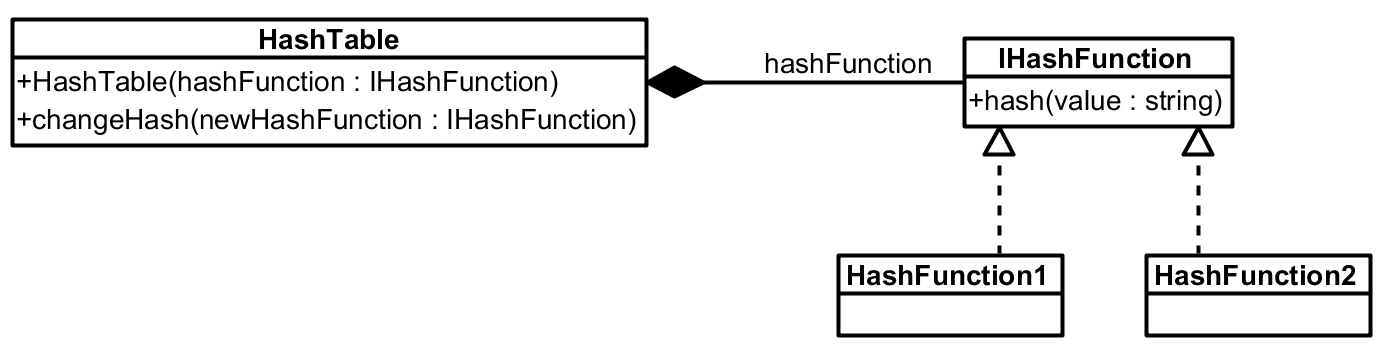
\includegraphics[width=0.9\textwidth]{modelExample.png}
		\end{center}
	\end{frame}

	\begin{frame}
		\frametitle{Язык UML}
		\begin{center}
			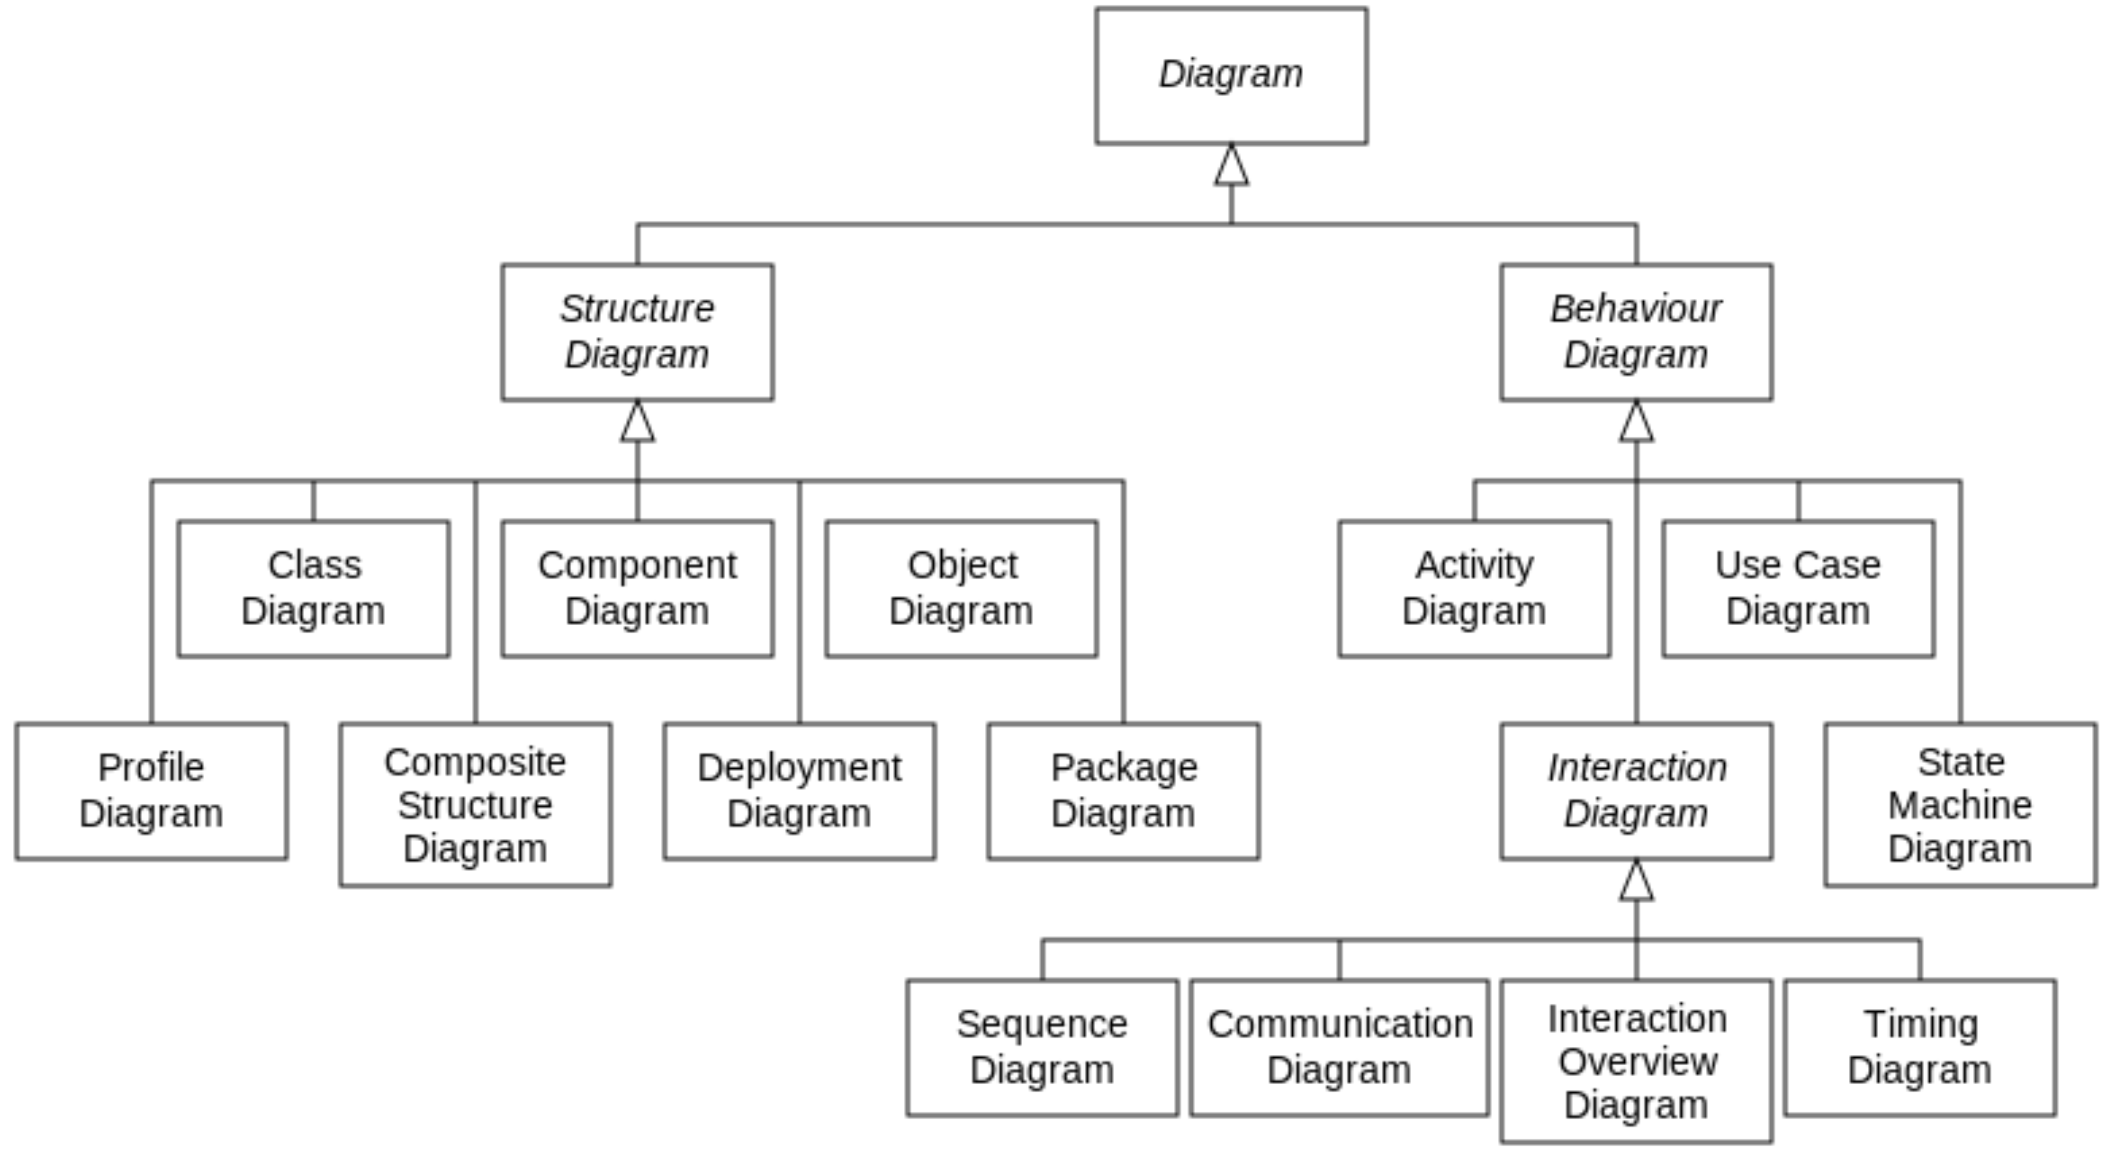
\includegraphics[width=0.9\textwidth]{umlDiagrams.png}
		\end{center}
	\end{frame}

	\begin{frame}
		\frametitle{Диаграммы классов UML}
		\begin{center}
			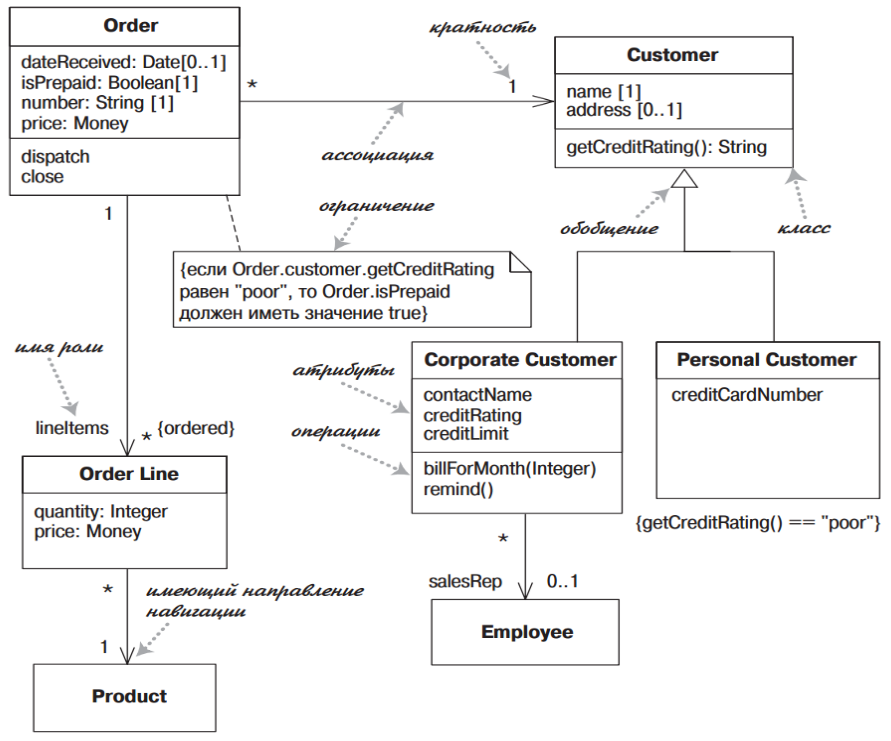
\includegraphics[width=0.7\textwidth]{umlClassDiagram.png}
		\end{center}
	\end{frame}

	\begin{frame}
		\frametitle{Свойства}
		\begin{columns}
			\begin{column}{0.3\textwidth}
				\begin{center}
					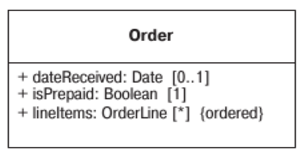
\includegraphics[width=0.8\textwidth]{attributes.png}

					Атрибуты
				\end{center}
			\end{column}
			\begin{column}{0.7\textwidth}
				\begin{center}
					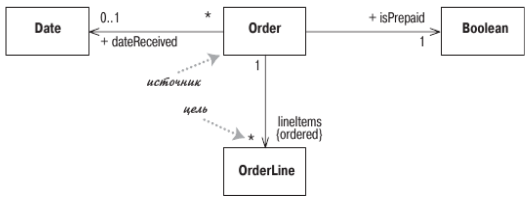
\includegraphics[width=0.7\textwidth]{associations.png}

					Ассоциации
				\end{center}
			\end{column}
		\end{columns}
		\bigskip
		Синтаксис:
		\begin{itemize}
			\item видимость имя: тип кратность = значение по умолчанию \{строка свойств\}
			\item Видимость: + (public), - (private), \# (protected), \char`~ (package)
			\item Кратность: 1 (ровно 1 объект), 0..1 (ни одного или один),\newline * (сколько угодно), 1..*, 2..*
		\end{itemize}
	\end{frame}

	\begin{frame}
		\frametitle{Агрегация и композиция}
		Агрегация – объект ``знает'' о другом (не управляет его временем жизни, имеет на него ссылку или указатель)
		\begin{center}
			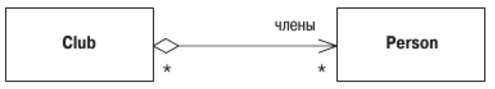
\includegraphics[width=0.5\textwidth]{aggregations.png}
		\end{center}
		Композиция --- объект владеет другим объектом (управляет его временем жизни, хранит его по значению или по указателю, делая delete)
		\begin{center}
			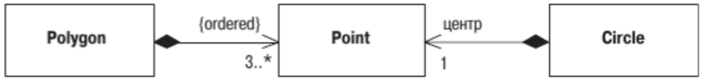
\includegraphics[width=0.7\textwidth]{compositions.png}
		\end{center}
		Уточнение обычной ассоциации, используется только если очень надо
	\end{frame}

	\begin{frame}
		\frametitle{Прочее}
		\begin{columns}
			\begin{column}{0.5\textwidth}
				\begin{center}
					Интерфейсы

					\bigskip
					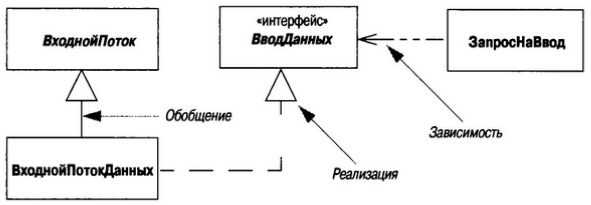
\includegraphics[width=0.9\textwidth]{interfaces1.png}

					\bigskip
					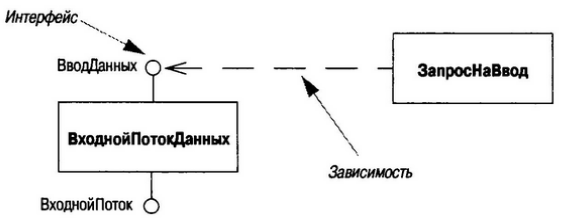
\includegraphics[width=0.9\textwidth]{interfaces2.png}
				\end{center}
			\end{column}
			\begin{column}{0.5\textwidth}
				\begin{center}
					Зависимости

					\bigskip
					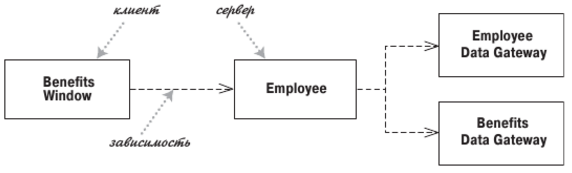
\includegraphics[width=0.9\textwidth]{dependencies.png}
					\bigskip

					Шаблоны

					\bigskip
					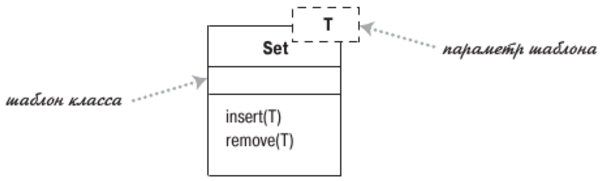
\includegraphics[width=0.9\textwidth]{templates.png}
				\end{center}
			\end{column}
		\end{columns}
	\end{frame}

	\begin{frame}
		\frametitle{Диаграммы компонентов}
		\framesubtitle{Component diagrams}
		\begin{center}
			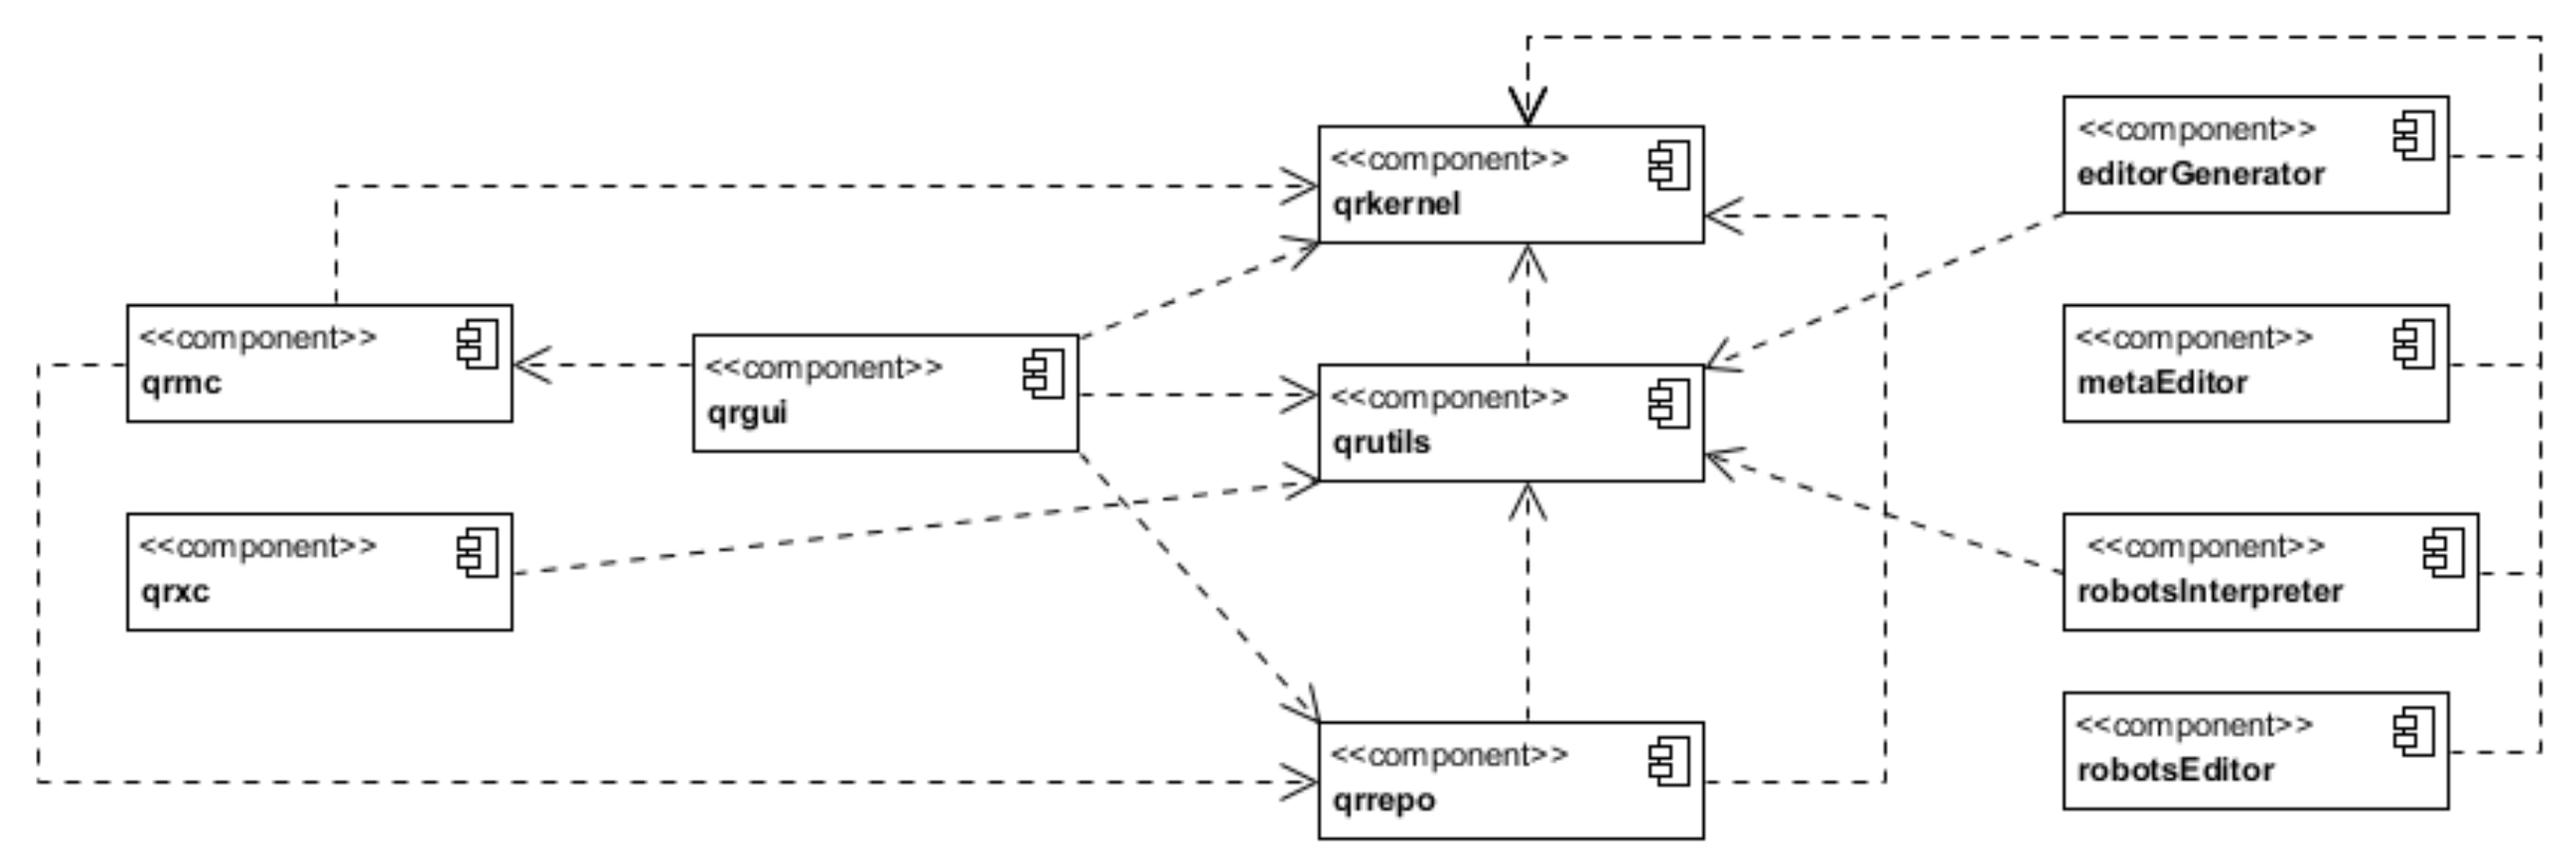
\includegraphics[width=0.9\textwidth]{componentDiagram.png}
		\end{center}
	\end{frame}

	\begin{frame}
		\frametitle{Диаграммы случаев использования}
		\framesubtitle{Use case diagrams}
		\begin{center}
			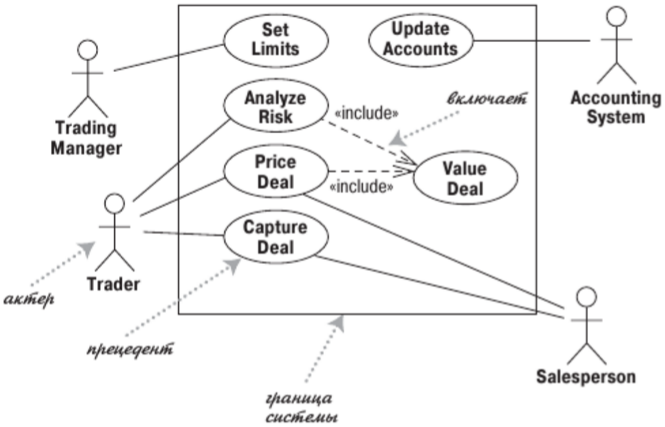
\includegraphics[width=0.6\textwidth]{useCaseDiagram.png}
		\end{center}
	\end{frame}

	\begin{frame}
		\frametitle{Диаграммы активностей}
		\framesubtitle{Activity diagrams}
		\begin{center}
			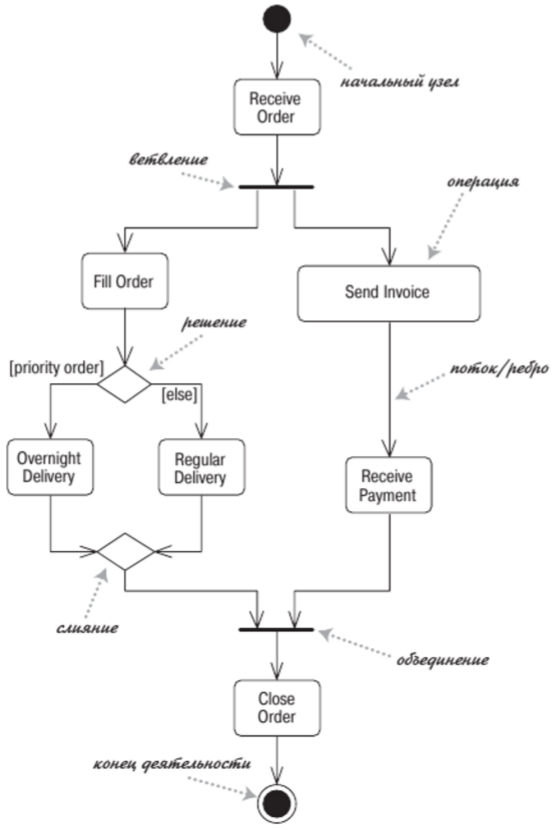
\includegraphics[width=0.415\textwidth]{activityDiagram.png}
		\end{center}
	\end{frame}

	\begin{frame}
		\frametitle{Диаграммы активностей, разделы}
		\framesubtitle{Swimlanes}
		\begin{center}
			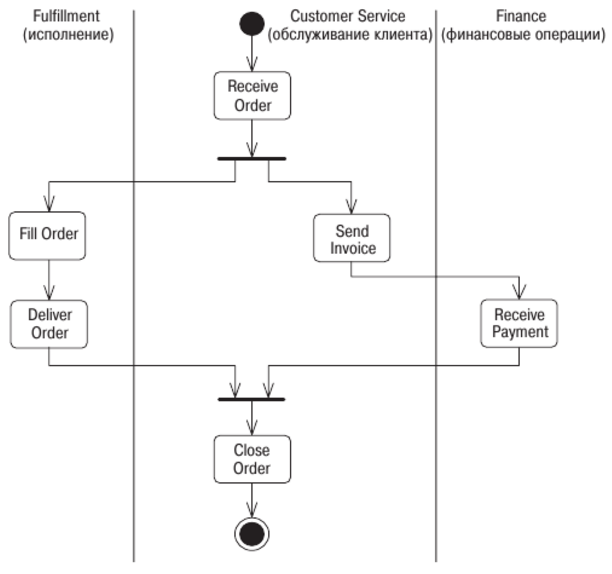
\includegraphics[width=0.55\textwidth]{activitySwimlanes.png}
		\end{center}
	\end{frame}

	\begin{frame}
		\frametitle{Диаграммы последовательностей}
		\framesubtitle{Sequence diagrams}
		\begin{center}
			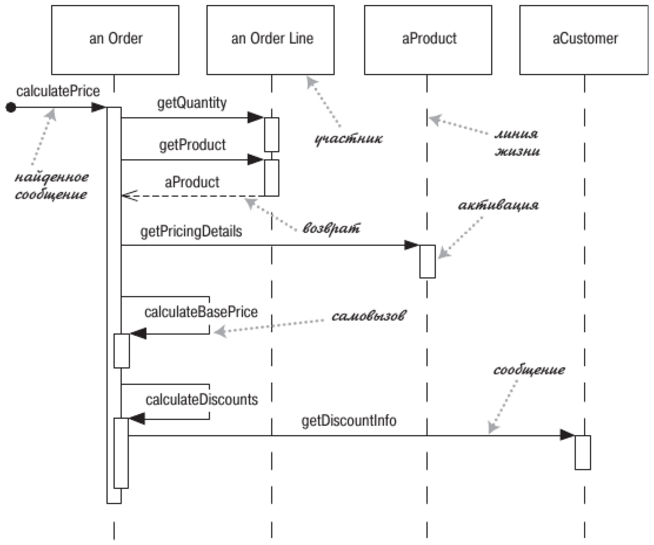
\includegraphics[width=0.6\textwidth]{sequenceDiagram.png}
		\end{center}
	\end{frame}

	\begin{frame}
		\frametitle{Диаграммы последовательностей, создание и удаление объектов}
		\begin{center}
			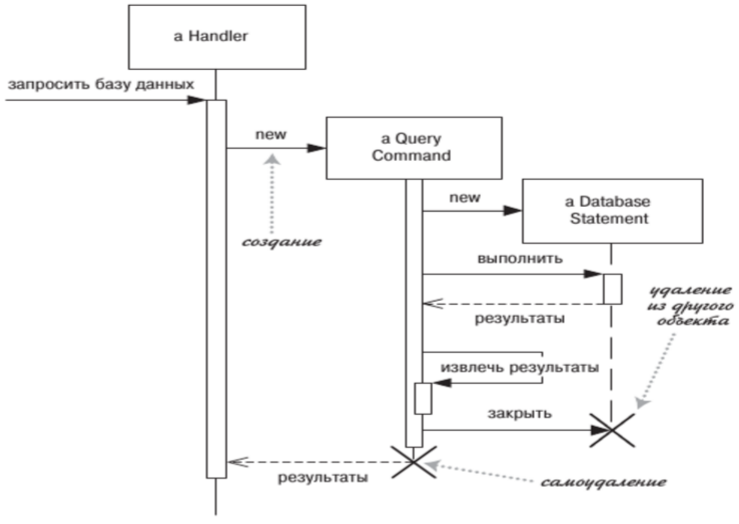
\includegraphics[width=0.65\textwidth]{sequenceLifeCycle.png}
		\end{center}
	\end{frame}

	\begin{frame}
		\frametitle{Диаграммы последовательностей, фреймы}
		\begin{center}
			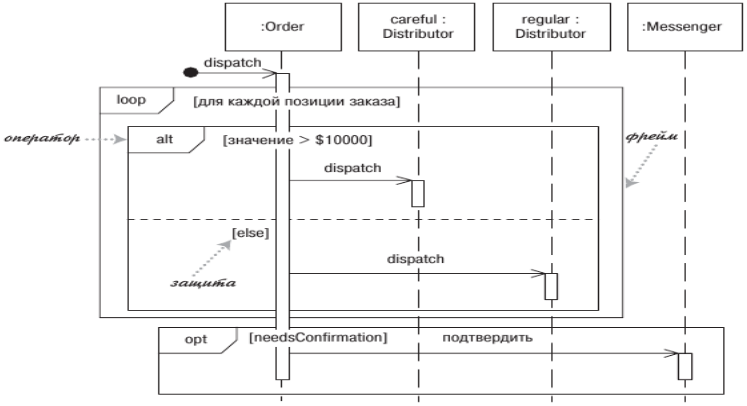
\includegraphics[width=0.8\textwidth]{sequenceFrames.png}
		\end{center}
	\end{frame}

	\begin{frame}
		\frametitle{Диаграммы конечных автоматов}
		\framesubtitle{State diagrams}
		\begin{columns}
			\begin{column}{0.5\textwidth}
				\begin{itemize}
					\item Состояние
					\begin{itemize}
						\item entry activity
						\item exit activity
						\item do activity
						\item внутренний переход
					\end{itemize}
					\item Событие
					\item Переход
					\begin{itemize}
						\item имя события (список параметров) [сторожевое условие] выражение действия
					\end{itemize}
				\end{itemize}
			\end{column}
			\begin{column}{0.5\textwidth}
				\begin{center}
					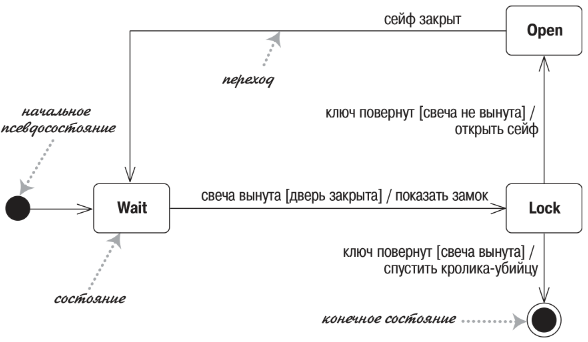
\includegraphics[width=\textwidth]{stateTransitionSyntax.png}
					\attribution{М. Фаулер, UML. Основы}
				\end{center}
			\end{column}
		\end{columns}
	\end{frame}

	\begin{frame}
		\frametitle{Диаграммы развёртывания}
		\framesubtitle{Deployment diagrams}
		\begin{columns}
			\begin{column}{0.5\textwidth}
				\begin{itemize}
					\item Показывает отображение компонентов и физических артефактов на реальные (или виртуальные) устройства
					\item Бывает полезна на начальных этапах проектирования, даже до диаграмм компонентов
				\end{itemize}
			\end{column}
			\begin{column}{0.5\textwidth}
				\begin{center}
					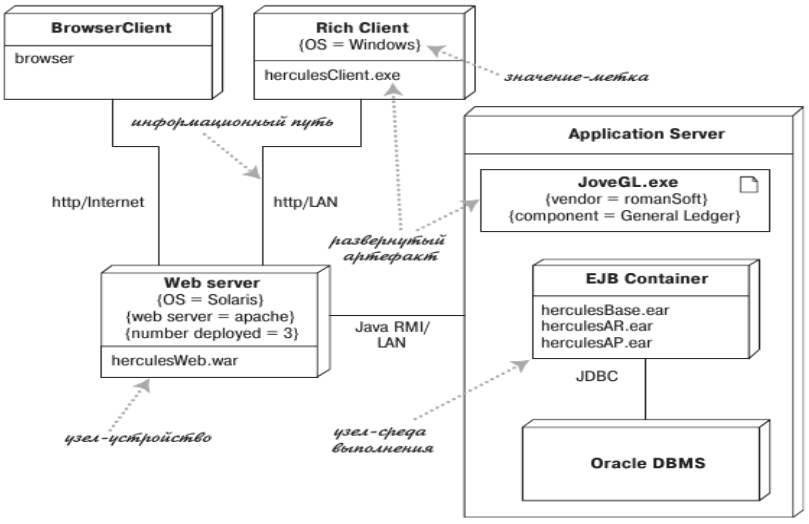
\includegraphics[width=\textwidth]{deploymentDiagram.png}
					\attribution{М. Фаулер, UML. Основы}
				\end{center}
			\end{column}
		\end{columns}
	\end{frame}

	\begin{frame}
		\frametitle{Предметно-ориентированные языки}
		\begin{center}
			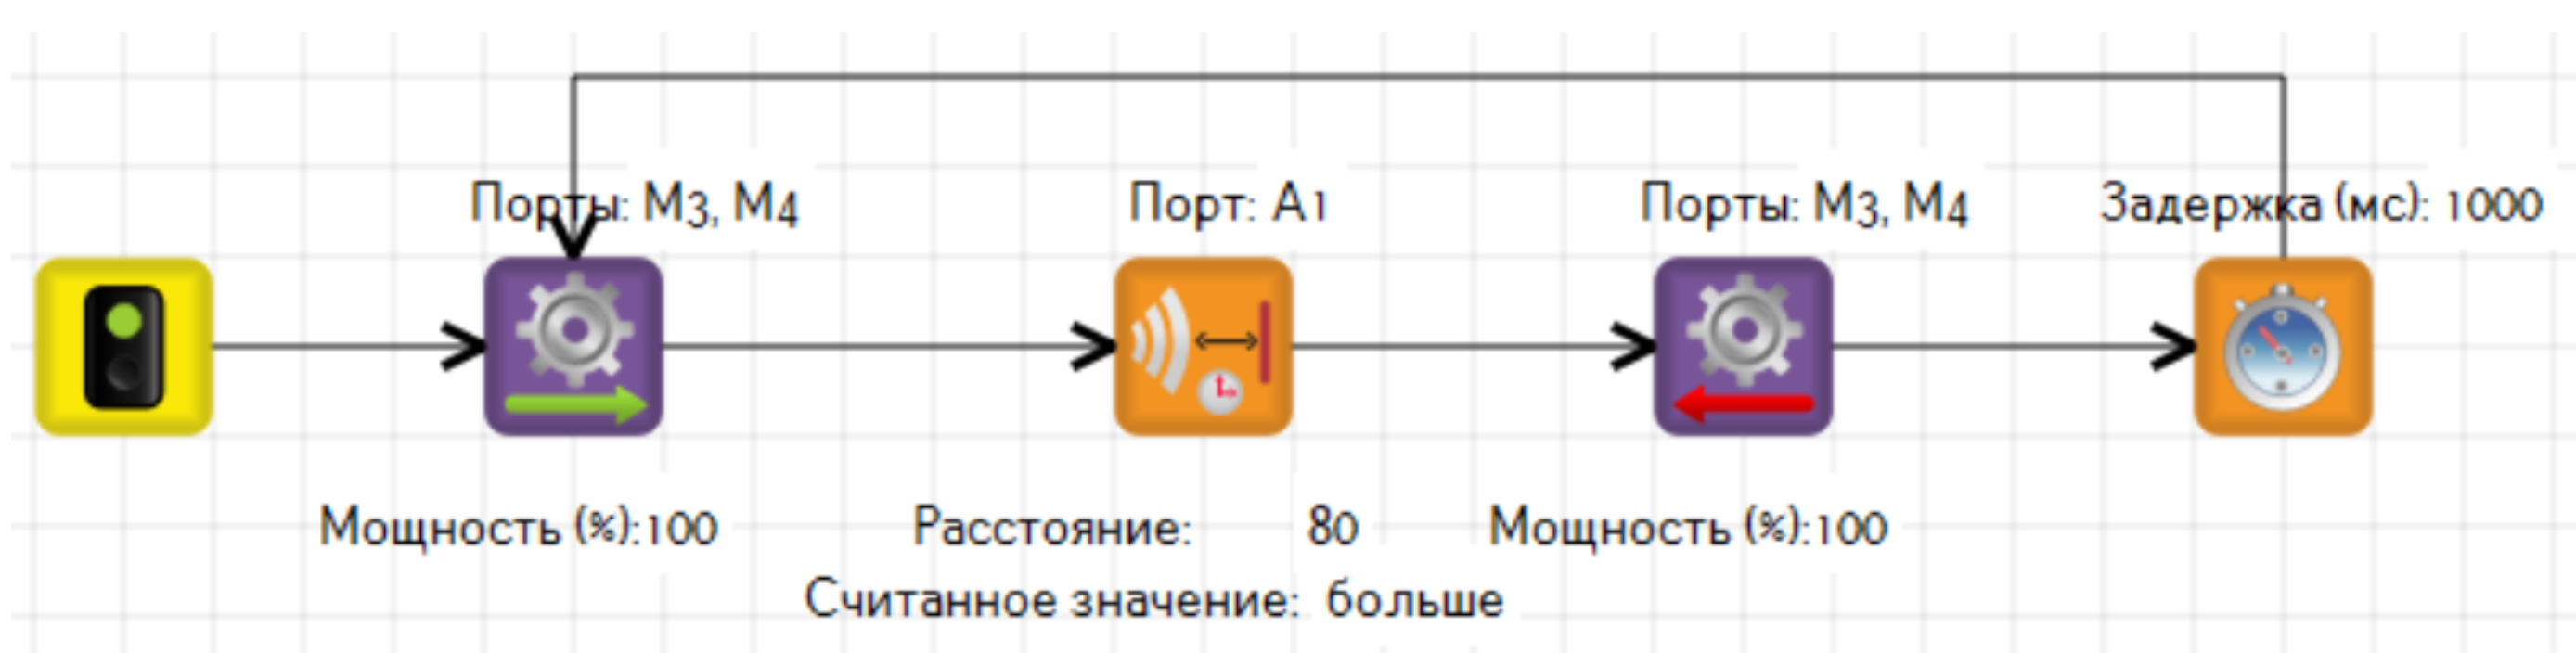
\includegraphics[width=0.9\textwidth]{domainLanguages.png}
		\end{center}
	\end{frame}

\end{document}
